\chapter{Load Balancing} \label{chapter:load_balancing} 
% Hilbert curve
% Hilbert state "guess"
% MPI transfers
% Non-conforming boundaries
% Reconstruction
% Say it only uses number of elements, point to results for N influence on GPUs
% Talk about load imbalance
% Talk about Hilbert state when splitting

A well made multi-block mesh can distribute the work evenly the different worker processes without
needing runtime adjustment if the topology and areas of more expensive computation stay the same
during the whole computation. This is complicated by the fact that, as seen in
Chapter~\ref{chapter:adaptive_mesh_refinement}, the mesh elements can increase their polynomial
order and split in multiple smaller elements in areas where the solution accuracy is not estimated
to be satisfactory. Unless the regions of interest happen to be evenly distributed between the
different processes, this will lead to an imbalance as some processes are left with more elements,
or higher-order elements, within their domain.

\begin{figure}[H]
	\centering
	\subfloat[Mesh before refining]
	{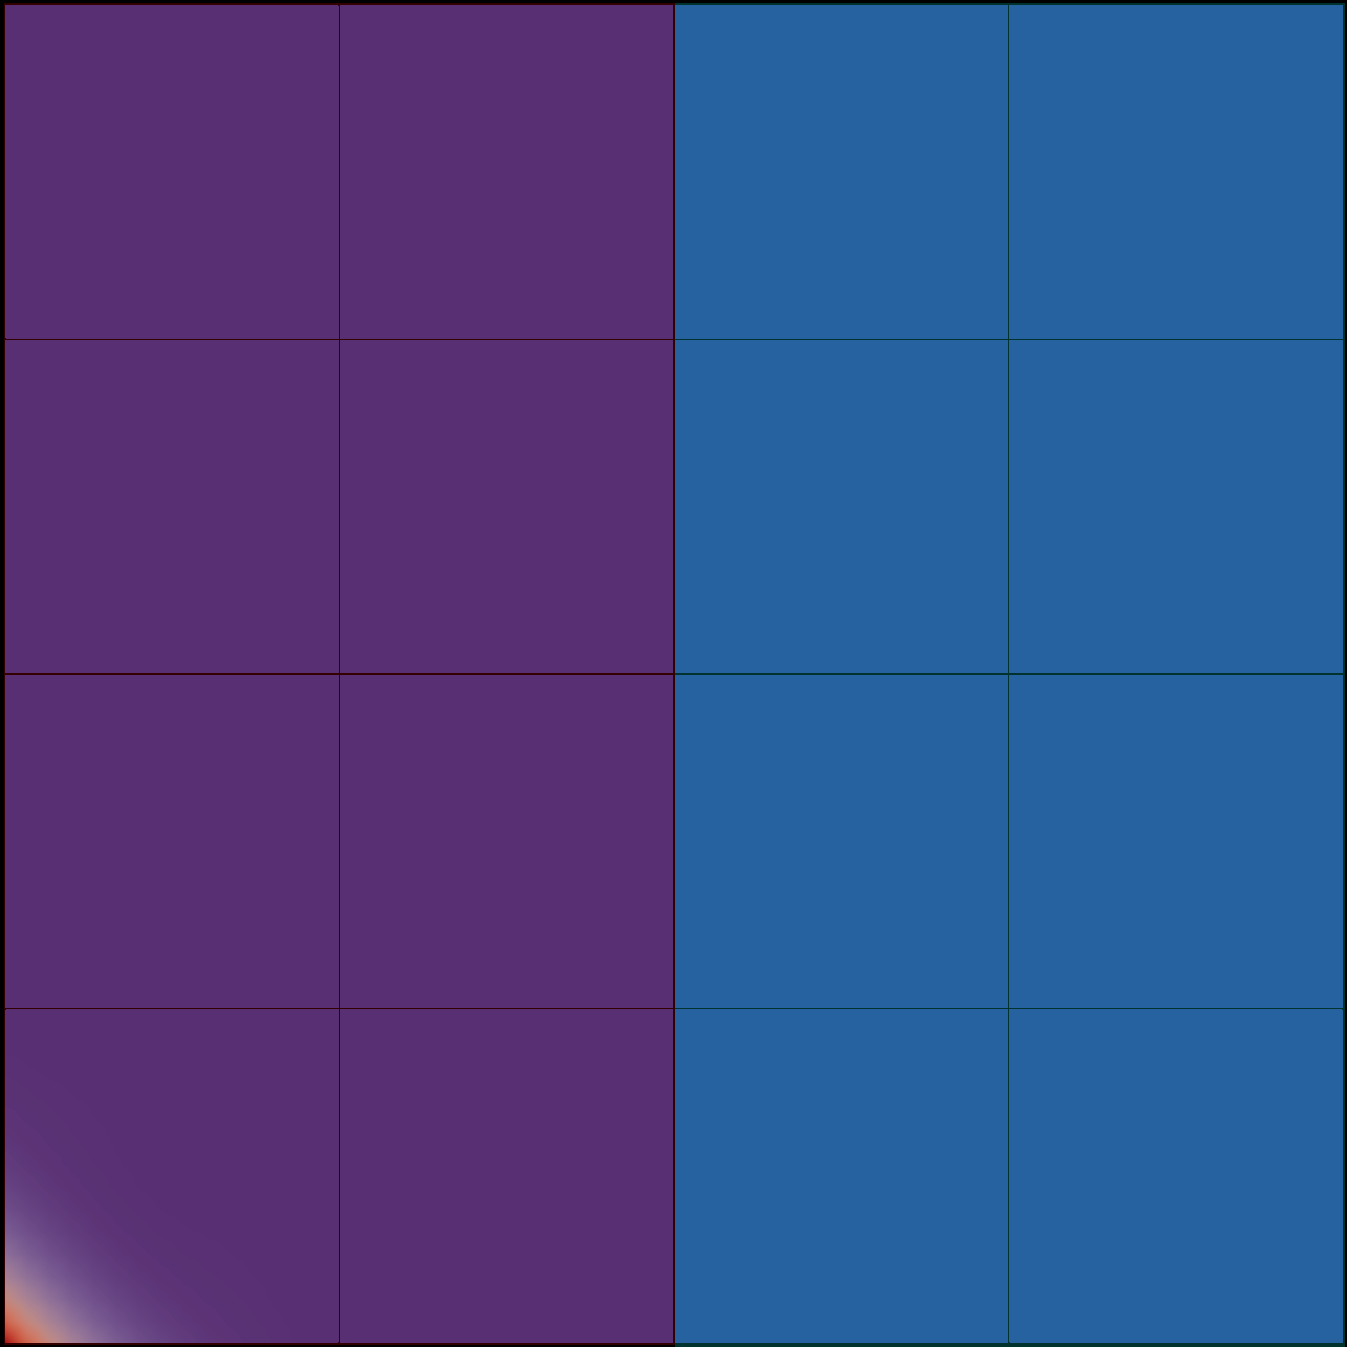
\includegraphics[width=0.45\textwidth]{Chapter_load_balancing/media/load_imbalance_initial} \label{fig:mesh_imbalance_initial_lb}}
	\hfill
	\subfloat[Mesh after refining]
	{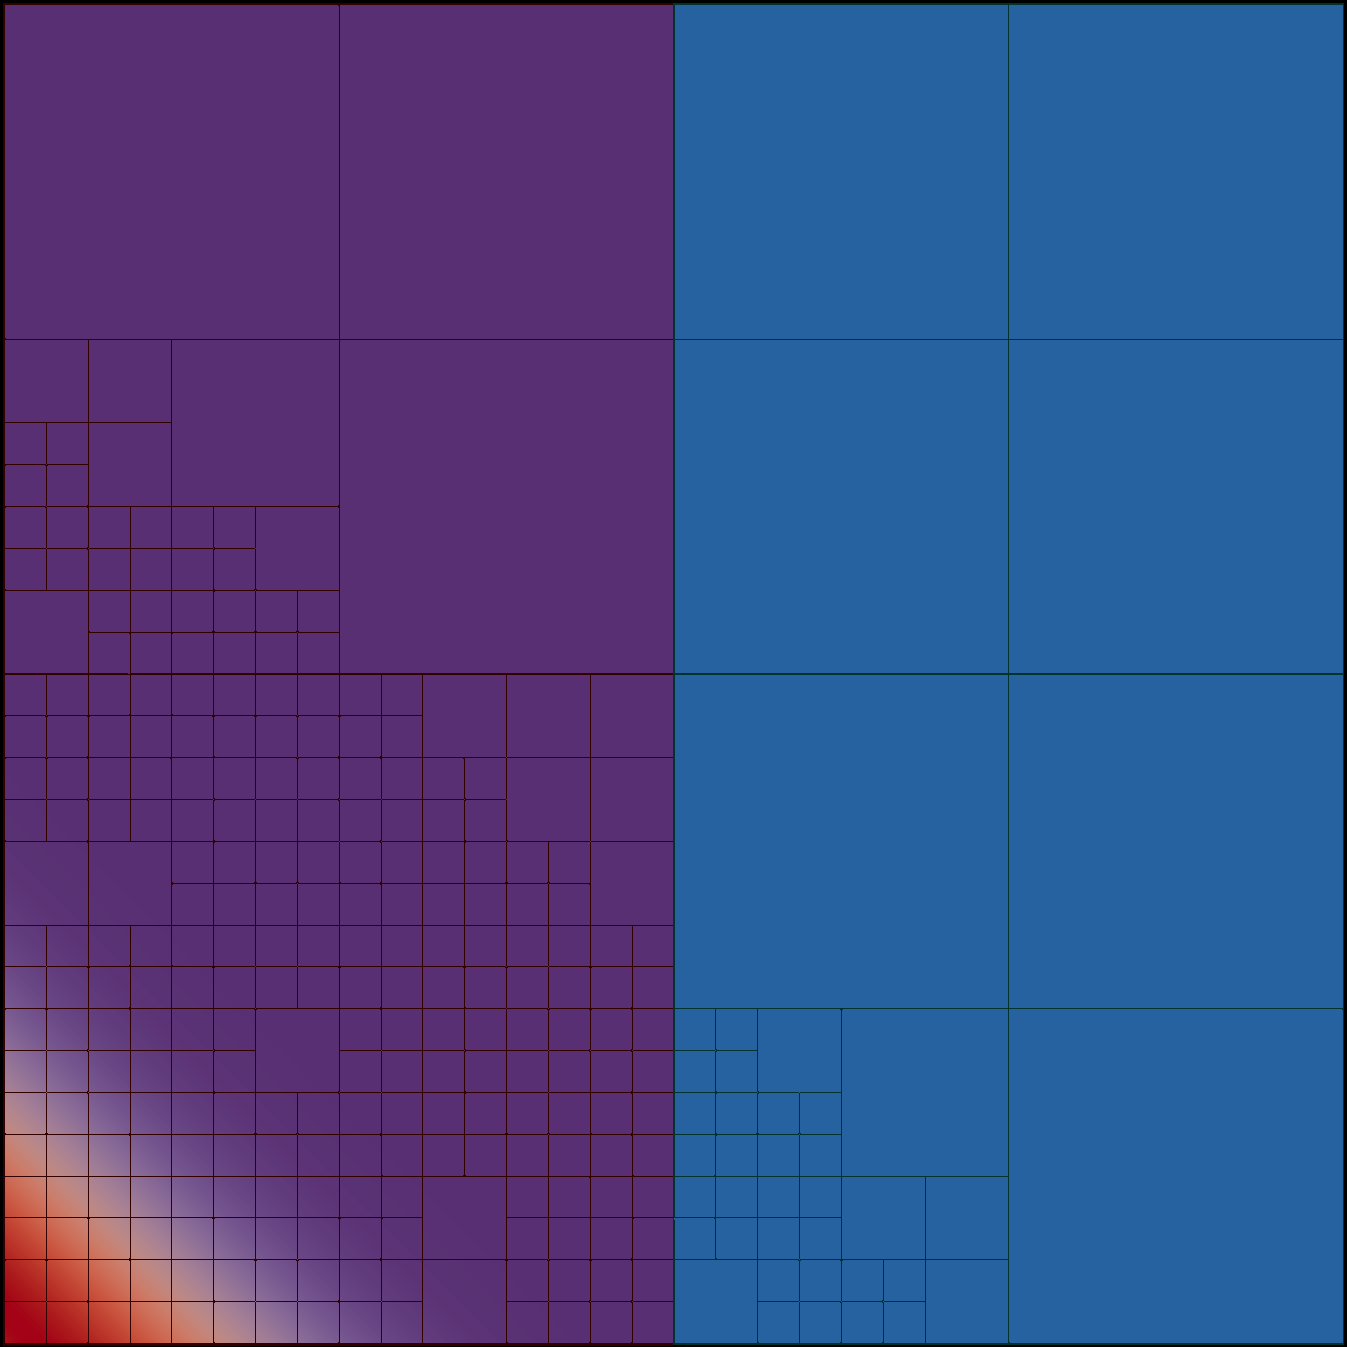
\includegraphics[width=0.45\textwidth]{Chapter_load_balancing/media/load_imbalance} \label{fig:mesh_imbalance_after_refinement_lb}}
	\caption{Load imbalance: The elements have split unequally in the two worker GPUs, one having a higher computational load. (a) Before refining (b) After refining}
	\label{fig:load_imbalance_lb}
\end{figure}

The wall time of the simulation will be driven by the most highly-loaded process, as the processes
have to synchronise at each time step. The less-loaded processes will simply wait for the other to
finish computing.

In order to keep good performance as the mesh is refined, we will need to perform dynamic load
balancing. Dynamic load balancing seeks to even out the computational load between the different
processes. The algorithm needs to be fast, to be executed often and keep the mesh optimal longer
without overshadowing the solving time. The worker processes in this work use GPUs for their
computations. Because transfers between GPUs are expensive, the algorithm needs to limit transfers
both during the load balancing process and during computation afterwards. The workers are made up of
one CPU core and one entire GPU. This means that the worker's processing power is mostly generated
by the GPU, and the algorithm needs to use it as much as possible. The algorithm will need t have
as mny parts as possible running on the GPU, in parallel. Finally, the algorithm needs to use as
little additional GPU memory as possible, as these processors have limited memory, especially
compared to CPUs.

The algorithm needs to select which elements to send from one GPU to another. Here, the
repartitioning scheme uses Space-Filling Curves (SFC), more specifically the Hilbert Curve. SFCs map
multi-dimensional space to one-dimensional space. Elements can then be sent or received from the
ends of this space. In addition, these curves are fast to generate, use low memory, and maximise
locality. Elements that are close in curve space will also be close by in the space used for
computations. This limits the number of interfaces between processes.

\section{Hilbert curve} \label{section:load_balancing:hilbert_curve}
% How adaptivity uses state
% Initial guess

\section{Reconstruction} \label{section:load_balancing:reconstruction}


\section{Implementation} \label{section:load_balancing:implementation}
\subsection{Element exchange} \label{section:load_balancing:implementation:element_exchange}
% and MPI datatype